%\documentclass[tikz,convert={outfile=\jobname.pdf}]{standalone}
\documentclass[tikz,convert={density=300,size=1080x800,outext=.png}]{standalone}

%\usetikzlibrary{calc,shape}
%\usetikzlibrary{...}% tikz package already loaded by 'tikz' option

\usepackage{xcolor}
\colorlet{water}{blue!10!white}
\colorlet{porousmedia}{brown!40!white}
\colorlet{Interface}{green!70!black}
\colorlet{slipwall}{orange!100!black}
\colorlet{noslipwall}{orange!100!black}


\begin{document}
  
%  \newcommand*{\Length}{1}
%  \newcommand{\channelHeight}{0.5*\Length}
  
  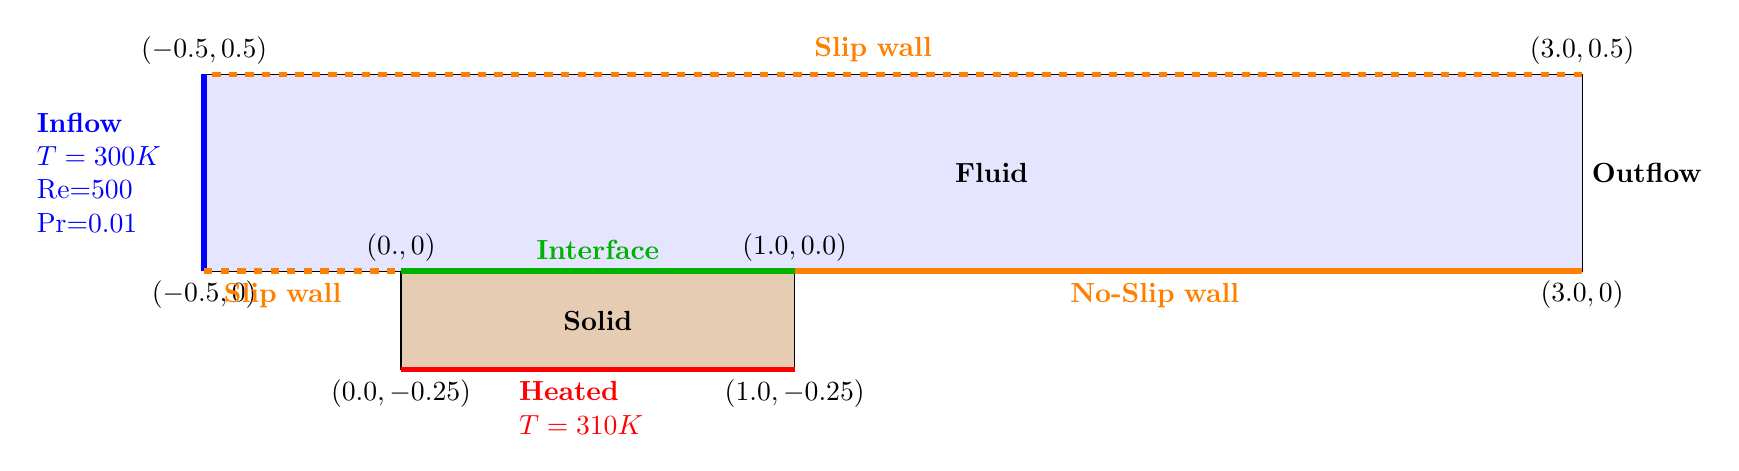
\begin{tikzpicture}[scale=5.0]% Example:
  
  \coordinate (fluid_n1) at (-0.5,0.0);
  \coordinate (fluid_n2) at (3.0,0.0);
  \coordinate (fluid_n3) at (3.0,0.5);
  \coordinate (fluid_n4) at (-0.5,0.5);
  
  \draw[fill=water] (fluid_n1) -- (fluid_n2) -- node[right, midway] {\textbf{Outflow}} (fluid_n3) -- (fluid_n4) -- node[color=blue,left, midway,text width=2cm] {\textbf{Inflow}\\$T=300K$\\Re=500\\Pr=0.01} (fluid_n1) ;
  
  \node[] at (1.5,0.25) {\textbf{Fluid}} ;
  
  \node[below] at (fluid_n1) {$(-0.5,0)$};
  \node[below] at (fluid_n2) {$(3.0,0)$};
  \node[above] at (fluid_n3) {$(3.0,0.5)$};
  \node[above] at (fluid_n4) {$(-0.5,0.5)$};
  
  \draw[color=blue,line width=2pt] (fluid_n1) -- (fluid_n4) node[right,midway, text width=2cm] {};
  
  
  \coordinate (solid_n1) at (0.0,0.0);
  \coordinate (solid_n2) at (0.0,-0.25);
  \coordinate (solid_n3) at (1.0,-0.25);
  \coordinate (solid_n4) at (1.0,0.0);
  
  \draw[fill=porousmedia] (solid_n1) -- (solid_n2) -- (solid_n3) -- (solid_n4) -- cycle;
  
  \node[above] at (solid_n1) {$(0.,0)$};
  \node[below] at (solid_n2) {$(0.0,-0.25)$};
  \node[below] at (solid_n3) {$(1.0,-0.25)$};
  \node[above] at (solid_n4) {$(1.0,0.0)$};
  
  \node[] at (0.5,-0.125) {\textbf{Solid}} ;
  
  \draw[color=Interface,line width=2pt] (solid_n1) -- (solid_n4) node[midway, above] {\textbf{Interface}};
  
  \draw[color=red,line width=2pt] (solid_n2) -- (solid_n3) node[midway, below, text width=2cm] {\textbf{Heated}\\$T=310K$};
  
%  Slipwall
  \draw[color=slipwall,line width=2pt, dashed] (fluid_n1) -- (solid_n1) node[below,midway, text width=2cm] {\textbf{Slip wall}};
  \draw[color=slipwall,line width=2pt, dashed] (fluid_n3) -- (fluid_n4) node[above,midway, text width=2cm] {\textbf{Slip wall}};
  
%  Noslip wall
  \draw[color=noslipwall,line width=2pt] (solid_n4) -- (fluid_n2) node[below,midway, text width=3cm] {\textbf{No-Slip wall}};
  
  \end{tikzpicture}
\end{document}